\documentclass[tikz,border=3pt]{standalone}
\usepackage[T1]{fontenc}
\usepackage{mathptmx}
\usepackage{tikz,pgfplots}
\usetikzlibrary{arrows.meta,positioning,calc,fit,backgrounds,shapes.geometric}
\pgfplotsset{compat=1.18}
\definecolor{forest}{HTML}{346E57}
\definecolor{sage}{HTML}{E8EFEA}
\definecolor{clay}{HTML}{AC653F}
\definecolor{sand}{HTML}{F4EAE2}
\definecolor{ink}{HTML}{252525}
\definecolor{light}{HTML}{F5F5F3}
\definecolor{gridgray}{HTML}{D8DAD6}
\tikzset{box/.style={draw=ink!70,line width=.5pt,rectangle,rounded corners=1pt,fill=white,align=center,font=\fontsize{11}{12}\selectfont,inner sep=6pt}, flow/.style={-{Latex[length=2.4mm]},line width=.7pt,draw=ink!80}, data/.style={flow,densely dashed,draw=forest}, label/.style={font=\fontsize{10}{11}\selectfont,fill=white,inner sep=2pt,align=center}}
\hyphenpenalty=10000\exhyphenpenalty=10000\begin{document}
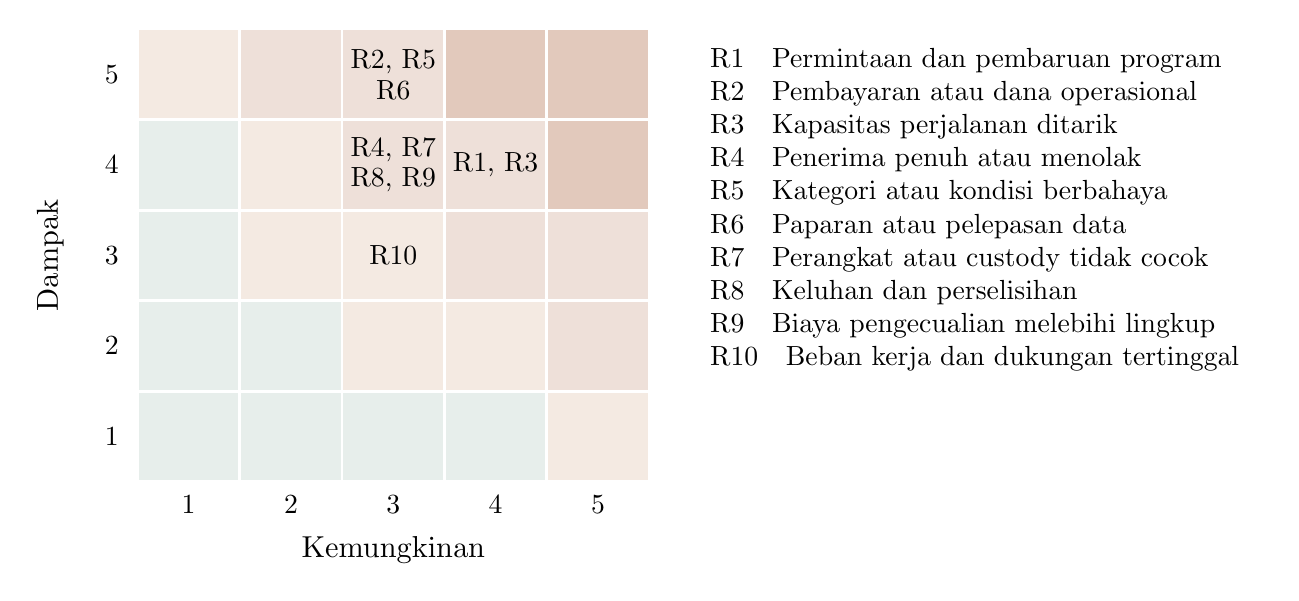
\begin{tikzpicture}[x=1.30cm,y=1.15cm]
\fill[forest!12](0,0)rectangle(1,1);\draw[white,line width=1pt](0,0)rectangle(1,1);
\fill[forest!12](0,1)rectangle(1,2);\draw[white,line width=1pt](0,1)rectangle(1,2);
\fill[forest!12](0,2)rectangle(1,3);\draw[white,line width=1pt](0,2)rectangle(1,3);
\fill[forest!12](0,3)rectangle(1,4);\draw[white,line width=1pt](0,3)rectangle(1,4);
\fill[sand](0,4)rectangle(1,5);\draw[white,line width=1pt](0,4)rectangle(1,5);
\fill[forest!12](1,0)rectangle(2,1);\draw[white,line width=1pt](1,0)rectangle(2,1);
\fill[forest!12](1,1)rectangle(2,2);\draw[white,line width=1pt](1,1)rectangle(2,2);
\fill[sand](1,2)rectangle(2,3);\draw[white,line width=1pt](1,2)rectangle(2,3);
\fill[sand](1,3)rectangle(2,4);\draw[white,line width=1pt](1,3)rectangle(2,4);
\fill[clay!20](1,4)rectangle(2,5);\draw[white,line width=1pt](1,4)rectangle(2,5);
\fill[forest!12](2,0)rectangle(3,1);\draw[white,line width=1pt](2,0)rectangle(3,1);
\fill[sand](2,1)rectangle(3,2);\draw[white,line width=1pt](2,1)rectangle(3,2);
\fill[sand](2,2)rectangle(3,3);\draw[white,line width=1pt](2,2)rectangle(3,3);
\fill[clay!20](2,3)rectangle(3,4);\draw[white,line width=1pt](2,3)rectangle(3,4);
\fill[clay!20](2,4)rectangle(3,5);\draw[white,line width=1pt](2,4)rectangle(3,5);
\fill[forest!12](3,0)rectangle(4,1);\draw[white,line width=1pt](3,0)rectangle(4,1);
\fill[sand](3,1)rectangle(4,2);\draw[white,line width=1pt](3,1)rectangle(4,2);
\fill[clay!20](3,2)rectangle(4,3);\draw[white,line width=1pt](3,2)rectangle(4,3);
\fill[clay!20](3,3)rectangle(4,4);\draw[white,line width=1pt](3,3)rectangle(4,4);
\fill[clay!35](3,4)rectangle(4,5);\draw[white,line width=1pt](3,4)rectangle(4,5);
\fill[sand](4,0)rectangle(5,1);\draw[white,line width=1pt](4,0)rectangle(5,1);
\fill[clay!20](4,1)rectangle(5,2);\draw[white,line width=1pt](4,1)rectangle(5,2);
\fill[clay!20](4,2)rectangle(5,3);\draw[white,line width=1pt](4,2)rectangle(5,3);
\fill[clay!35](4,3)rectangle(5,4);\draw[white,line width=1pt](4,3)rectangle(5,4);
\fill[clay!35](4,4)rectangle(5,5);\draw[white,line width=1pt](4,4)rectangle(5,5);
\foreach\n in{1,...,5}{\node[font=\fontsize{10}{11}\selectfont]at(\n-.5,-.25){\n};\node[font=\fontsize{10}{11}\selectfont]at(-.25,\n-.5){\n};}
\node[font=\fontsize{11}{12}\selectfont]at(2.5,-.75){Kemungkinan};\node[font=\fontsize{11}{12}\selectfont,rotate=90]at(-.85,2.5){Dampak};
\node[align=center,font=\fontsize{10}{11}\selectfont]at(3.5,3.5){R1, R3};
\node[align=center,font=\fontsize{10}{11}\selectfont]at(2.5,4.5){R2, R5\\R6};
\node[align=center,font=\fontsize{10}{11}\selectfont]at(2.5,3.5){R4, R7\\R8, R9};
\node[align=center,font=\fontsize{10}{11}\selectfont]at(2.5,2.5){R10};
\node[anchor=north west,font=\fontsize{10}{12}\selectfont,text width=7cm]at(5.5,4.9){R1\quad Permintaan dan pembaruan program\\R2\quad Pembayaran atau dana operasional\\R3\quad Kapasitas perjalanan ditarik\\R4\quad Penerima penuh atau menolak\\R5\quad Kategori atau kondisi berbahaya\\R6\quad Paparan atau pelepasan data\\R7\quad Perangkat atau custody tidak cocok\\R8\quad Keluhan dan perselisihan\\R9\quad Biaya pengecualian melebihi lingkup\\R10\quad Beban kerja dan dukungan tertinggal};
\end{tikzpicture}
\end{document}
